\section{Goal \label{sec:goal}}
Qualitatively speaking, the goal of suspension commissioning is simply to bring the suspensions into a state where interferometer commissioners can use the suspensions, via defined entry points, to steer the mirrors and make an interferometer, which is sensitive enough to be a gravitational wave detectors.
Althrough, as mentioned, there's no realistic requirements, which are derived from previous experience, we adopt theoretical requirements derived from \cite{Sekiguchi:2016bmv}. In particular, in order for KAGRA to function as an gravitational wave detector, the suspensions have to satisfied 2 types of requirements, displacement noise requirement, residual motion requirement.
In this section, we will briefly discuss the requirements, but will not go into the details, as this is not the scope of this document.
Readers are recommended to refer to the external references cited.

\subsection{Displacement noise requirement \label{sec:displacement_noise_requirement}}
Ground-based gravitational wave detectors have a detection band starting from $10~\mathrm{Hz}$.
The detectable effect of gravitational waves comes in the form of strain, which loosely speaking, is the fractional change in length.
To detect gravitational waves, we simply use an L-shape interferometer and measure the change in the arm lengths in two directions.
We expect targeted gravitational waves to have a peak amplitude of $10^{-21}$.
While the arm lengths of the interferometer are in the order of $10^{3}~\mathrm{m}$, the change in arm lengths caused by targeted gravitational wave is expected to be in the order of $10^{-21}\times 10^{3}~\mathrm{m}=10^{-18}~\mathrm{m}$, which is a very tiny amount of displacement.
Effectively, this means that the test masses (TM), i.e. the end mirrors, must have a displacement level lower than that.
Giving a safety factor of $10$, i.e. signal-to-noise ratio of around 100, this converts a displacement noise requirement of $10^{-19}~\mathrm{m}$ at $10~\mathrm{Hz}$, roughly speaking. Figure.~\ref{fig:displacementnoiserequirement} shows the displacement noise requirement of the optics including the test mass (TM), beamsplitter (BS), signal recycling mirror (SRM), and power recycling mirror (PRM) above $10~\mathrm{Hz}$.
\begin{figure}[!h]
	\centering
	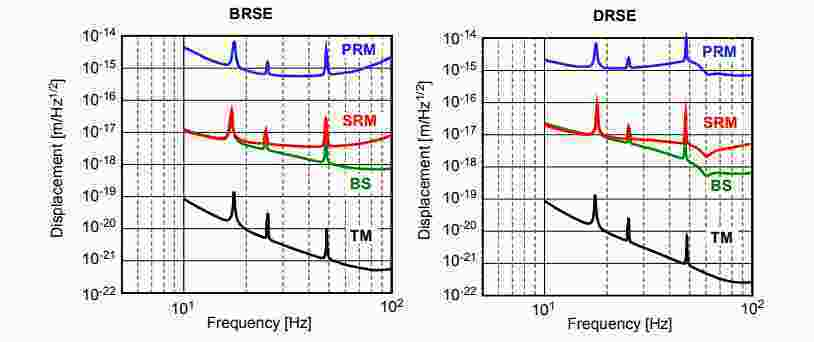
\includegraphics[width=0.7\linewidth]{figures/displacement_noise_requirement}
	\caption{Displacement noise requirements of the test mass (TM) (black), beamsplitter (BS) (green), signal recycling mirror (SRM) (red), and power recycling mirror (PRM) (blue), under boardband resonant sideband extraction configuration (BRSE) (Left) and detuned resonant sideband extraction scheme (DRSE) (Right). Retrieved from \cite{Sekiguchi:2016bmv}.}
	\label{fig:displacementnoiserequirement}
\end{figure}
As can be seen, the requirements of optics other than the TMs are much lower.
The displacement noise level of the BS and the SRM is at $10^{-17}~\mathrm{m}$, while that of the PRM is at $10^{-15}~\mathrm{m}$.
Table~.\ref{table:displacement_noise_requirement} summarizes the displacement noise of various optics at $10~\mathrm{Hz}$.
Therefore, the partial goal of suspension commissioning is to make sure these displacement noise levels requirement are met.
\begin{table}[!h]
	\centering
	\begin{tabular}{|c|c|}
		\hline
		& Displacement level ($\mathrm{m}/\sqrt{\mathrm{Hz}}$)\\
		\hline
		TM &  $1\times 10^{-19}$\\
		\hline
		BS &  $1\times 10^{-17}$\\
		\hline
		PRM & $2\times 10^{-15}$\\
		\hline
		PR2, PR3 & $1\times 10^{-15}$\\
		\hline
		SRM & $1\times 10^{-17}$\\
		\hline
		SR2, SR3 & $5\times 10^{-18}$\\
		\hline
	\end{tabular}
	\caption{Summary of longitudinal displacement noise level (at $10~\mathrm{Hz}$) of the optics including the folder mirrors of the recycling cavity (PR2, PR3, SR2, SR3). Retrieved from \cite{Sekiguchi:2016bmv}.}
	\label{table:displacement_noise_requirement}
\end{table}
The suspensions of the optics are designed specifically to attenuate the seismic noise at $10~\mathrm{Hz}$ to the displacement level specified in table.~\ref{table:displacement_noise_requirement} via passive isolation.
Therefore, the suspensions intrinsically satisfied these requirements already without any tweaking.
However, the main concern here is not about passive isolation.
Instead, it's about active isolation/feedback control, as we need to keep the control noise below these displacement level, while maintaining certain disturbance rejection capability.
This brings us to the other requirement: residual motion.

\subsection{Residual motion requirement \label{sec:residual_motion_requirement}}
In previous section, we discussed what are the requirements for KAGRA to be sensitive enough to become a gravitational wave detector.
Here, we will discuss the requirements for KAGRA to be an interferometric gravitational wave detector.
In particular, we will discuss velocity, angular fluctuation, and displacement level requirement.
Again, here we only briefly mention the rationale behind such requirements and readers are strongly recommended to read \cite{Sekiguchi:2016bmv} for detailed explanations.

\subsubsection{Residual velocity requirement}
In order for KAGRA to become an interferometric gravitational wave detector, the main optics must be manipulated to form various optical cavities, where feedback control is used to ``lock'' two mirrors at relatively stable separations.
The technique used is called Pound-Drever-Hall (PDH) technique \cite{doi:10.1119/1.1286663}.
To use this technique, the separation between two optics stay within the operating range where the control signal for using PDH technique becomes linear.
In \cite{Sekiguchi:2016bmv}, a velocity requirement of the is derived by considering the maximum actuation power of the TM coils.
Consider a case where the optics are moving towards the operating range.
As the optics enter the range, the actuators applies maximum force on the optics, causing the optics to decelerate maximally.
If the optics are put to halt before they exit the operating range, then lock-acquisition is achieved.
This only happens when the velocity of the optics is lower than a certain threshold, which we define as a requirement.
The velocity requirements the main optics are derived in \cite{Sekiguchi:2016bmv} and is summarized in table.~\ref{table:velocity_requirement}.
\begin{table}[!h]
	\centering
	\begin{tabular}{|c|c|}
		\hline
		& Velocity requirement (RMS) ($\mu\mathrm{m}/\mathrm{s}$)\\
		\hline
		TM, BS, SR &  $0.5$\\
		\hline
		PR &  $2$\\
		\hline
	\end{tabular}
	\caption{Summary of main optics' velocity requirement. Retrieved from \cite{Sekiguchi:2016bmv}.}
	\label{table:velocity_requirement}
\end{table}

\subsubsection{Residual angular displacement requirement}
Now, I don't really understand the rationale behind these angular fluctuation requirements\footnote{Please help me to write this section if you know the correction explanation. As far as I know, the angular fluctuation requirement comes from the fact that the interferometer needs to be aligned and that the beam spots are within good range around the center of the optics. But, I don't really know how people got those numbers.} and it seems that different sources suggests different things. I will simply report the requirements from some sources. 

In \cite{Sekiguchi:2016bmv}, it was reported that the RMS angles of the mirrors should not produce beam spot fluctuation on the optics by larger than an RMS value of $1~\mathrm{mm}$.
Using the beam paths as the lever arm, the angle fluctuation requirements are calculated and shown in table.~\ref{table:angular_fluctuation_requirement}.
\begin{table}[!h]
	\centering
	\begin{tabular}{|c|c|}
		\hline
		& Angular fluctuation RMS ($\mu\mathrm{rad}$)\\
		\hline
		TM &  $0.2$\cite{Sekiguchi:2016bmv, yuta_oplev}~/~$0.01$\cite{PhysRevD.88.043007, Mueller:05}\\
		\hline
		BS &  $4$\\
		\hline
		PRM & $45$\\
		\hline
		PR2 & $20$\\ 
		\hline
		PR3 & $2$\\
		\hline
		SRM & $25$\\
		\hline
		SR2 & $10$\\
		\hline
		SR3 & $1$\\
		\hline
	\end{tabular}
	\caption{Angular fluctuation requirements of the optics. Retrieved from \cite{Sekiguchi:2016bmv, yuta_oplev} unless otherwise specified.}
	\label{table:angular_fluctuation_requirement}
\end{table}
However, in another source regarding beam jittering at LIGO \cite{Mueller:05}, it's mentioned that the angular fluctuation requirement of the test masses at LIGO is $10^{-8}~\mathrm{rad}$.
The same value is also used to derive the wavefront sensor sensitivity requirement at KAGRA \cite{PhysRevD.88.043007}.
It's worth noting that both of these sources were also cited in \cite{Sekiguchi:2016bmv}.
So unless there's extra comment regarding this, let's just set the requirement for the TM to the lower one ($10^{-8}~\mathrm{rad}$) as a worst case scenario\footnote{There's a chance that we cannot confirm that we actually satisfied this requirement at the end of suspension commissioning as there's no sensors sensitive enough to measure such small level of fluctuation.Let's hope that our optical levers are sensitive enough}.

\subsubsection{Longitudinal displacement level requirement}
At last, the longitudinal displacement requirement was derived also from the maximum actuation power of the force coils at the TM stage.
Doing so, we assume that only these actuators are used during lock acquisition, but this may not be the case, so here again we are assuming a worst case scenario.
Table.~\ref{table:displacement_rms_requirement} summarizes the displacement RMS value requirement of the main optics in KAGRA.
\begin{table}[!h]
	\centering
	\begin{tabular}{|c|c|}
		\hline
		& Displacement RMS requirement ($\mu\mathrm{m}$)\\
		\hline
		TM &  $0.01$\\
		\hline
		BS &  $3.3$\\
		\hline
		SRM & $3.3$\\
		\hline
		SR2, SR3 & $1.6$\\
		\hline
		PRM & $560$\\
		\hline
		PR2, PR3 & $280$\\
		\hline
	\end{tabular}
	\caption{Longitudinal displacement RMS requirement of the optics. Retrieved from \cite{Sekiguchi:2016bmv}.}
	\label{table:displacement_rms_requirement}
\end{table}
This concludes the residual motion requirements for the core optics. 
So, the other half of the goal is to actively control the suspensions so requirements as shown in Table.~\ref{table:velocity_requirement}, \ref{table:angular_fluctuation_requirement}, and \ref{table:displacement_rms_requirement} are met, while not violating noise specification as shown in Table.~\ref{table:displacement_noise_requirement}.
In the following sections, we shall discuss/review some of the methods and techniques that can be used to achieve these goals.
We will also discuss some ways that we used to verify the satisfaction these requirements.

\subsection{Miscellaneous}
This section mainly refers to artificial requirements that are set in \cite{suspension_commissioning}.

\subsubsection{Seismic noise}
As a vibration isolation system, the main goal of the suspensions is to isolate the sole external disturbance, that is, the seismic disturbance.
Therefore, the optics must satisfy the displacement noise and residual motion requirements under the influence of a background seismic noise.
However, the residual motion of the optics vary with seismic noise level, which means that the performance of the suspension evaluated at a certain moment may not be the same at the other, as the seismic noise is dynamic.
So, we purpose an additional constraint here.
We require that the displacement noise and residual motion requirements to be satisfied under the influence of a disturbance equivalent to a background seismic noise at the $90^\mathrm{th}$ percentile level in the winter season.
The choice of this seismic noise meant to be conservative as it's considered a very violent disturbance.
To give some perspective of how the seismic noise level is, the seismic noise at the $90^\mathrm{th}$ percentile in KAGRA is shown in Fig.~\ref{fig:kagra_seismic_noise_90th_percentile} \cite{seismic_noise_kagra}.
\begin{figure}[!h]
	\centering
	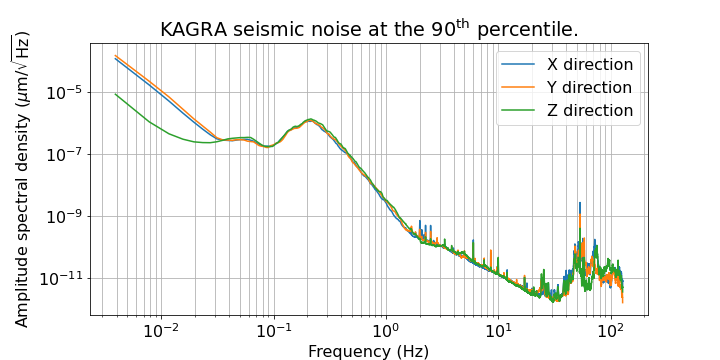
\includegraphics[width=0.7\linewidth]{figures/kagra_seismic_noise_90th_percentile.png}
	\caption{The amplitude spectral density of seismic noise in KAGRA at $90^\mathrm{th}$ percentile in $x$ (blue), $y$ (yellow), and $z$ (green) direction. Data retrieved from \cite{seismic_noise_kagra}.}
	\label{fig:kagra_seismic_noise_90th_percentile}
\end{figure}
As is mentioned, this is a conservative requirement, and it can be rare to observe such huge disturbance.
This means that it can be hard to test the suspension performance naturally.
To this end, as we shall see in later sections [ref later sections], we purpose to inject, using the actuators, artificial time series that has the same amplitude spectral density (ASD) of the measured seismic noise.

\subsubsection{Guardian}
Guardian is an automation system used in advanced LIGO (aLIGO) \cite{advanced_ligo_guardian}.
It's a platform where operators can program, using Python, certain operations that takes the suspensions from one defined states to another via certain defined paths.
The details of Guardian will not be discussed here, readers are strongly recommended to read the ``living'' document from aLIGO \cite{advanced_ligo_guardian}.
We will only briefly introduce what we're trying to achieve with Guardian and what people should expect.
Here, we will relay information given in \cite{suspension_commissioning, all_of_the_vibration}.
\begin{figure}[!h]
	\centering
	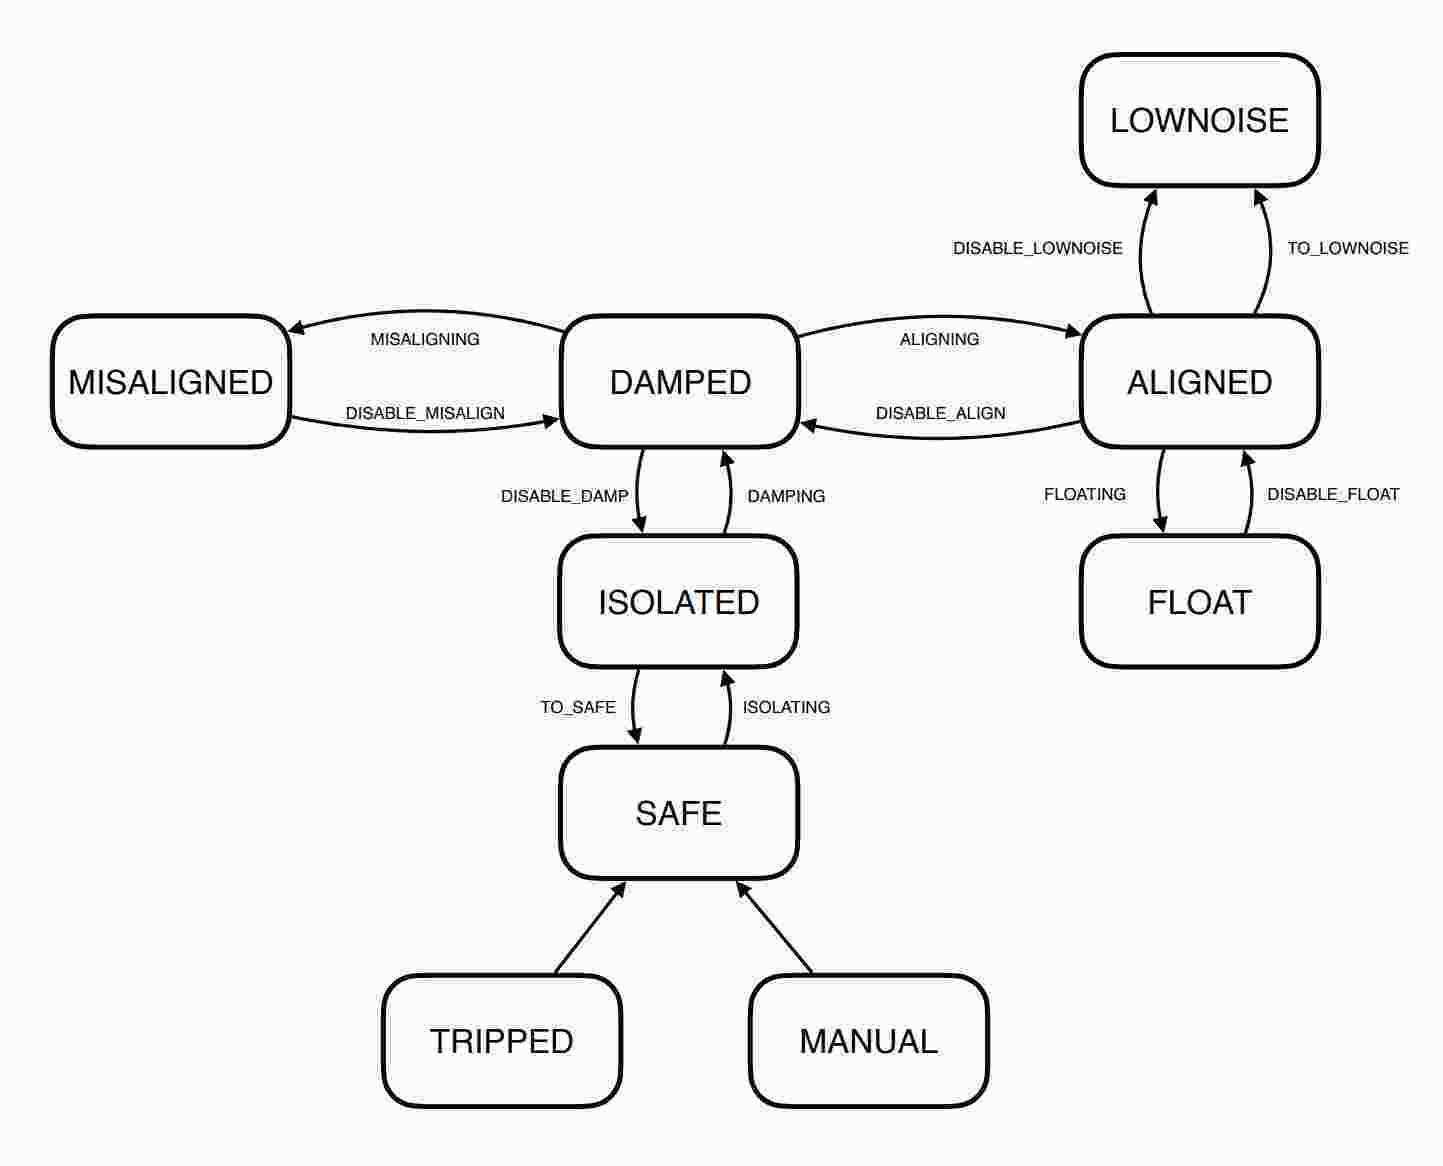
\includegraphics[width=0.7\linewidth]{figures/guardian}
	\caption{State-transition diagram of the (proposed?) VIS Guardian. Retrieved from \cite{all_of_the_vibration}}
	\label{fig:guardian}
\end{figure}
Fig.~\ref{fig:guardian} shows the (proposed?) state-transition diagram of the VIS Guardian.
As can be seen, there are 9 Guardian states, namely TRIPPED, MANUAL, SAFE, ISOLATED, DAMPED, MISALIGNED, ALIGNED, FLOATED, and LOWNOISE.
Here, description in \cite{all_of_the_vibration} is lacking so we will be further elaborating the behavior of these states.

In the TRIPPED state, as is indicated by the name of the state, the suspension is tripped.
This is triggered by a builtin watchdog system in the real-time model that monitors for abnormal behaviors.
The suspension can ``jump'' (In Guardian language) into this state from every other state.
This happens when the watchdog's tripped.

As for the MANUAL state, not sure what that means.
But my guess is that this is a state with the master switch turned on, so actuation signals can go through for measurement and diagnostic purposes.

In the SAFE state, actuation signals cannot go to the actuators, essentially immobilizing the suspension.

In the ISOLATED state, active isolation, usually at the stage closest to the ground (likely preisolator/inverted pendulum), is engaged.
The controls systems are engaged such that two things are achieved: 1) Coarsest alignment with integration action, and 2) Seismic noise suppression.
The controls at the higher stage will bring lower stages into operating point (e.g.centering the optical levers), but will perturb lower stage resonances via control noise injection.

In the DAMPED state, controls at the lower stages will be engage to suppress the these resonances.
At this point, the suspension should be able to satisfy the residual motion requirements as stated in Sec.~\ref{sec:residual_motion_requirement}.

In the ALIGNED state, the optics is steered to be coarsely aligned and is ready to be handed over to inferometer control.
Distinct from the ALIGN state, In the MISALIGN state, the optics is steered away from the aligned position.

At last, at the LOWNOISE state, controls that may compromise the detector sensitivity will be shut off or replaced by a lower noise version.
At this point, the suspension should satisfy the displacement noise requirements as stated in Sec.~\ref{sec:displacement_noise_requirement}.


